
\section{Method and Materials}

\subsection{Automatic Light Switching based on Visitor Count}

\begin{multicols}{2}

The main component used for automatic light switching is Ultrasonic
Sensor. The ultrasonic sensor is used to reckon the number of person
entering and exiting a room and determine the number of visitors.

The fundamental principle behind people counter is that two separate
US sensors are placed at the front and rear of the doorway such that
one sensor is proximal to the indoor and the other is proximal to the
outdoor as show in the following diagram:
\begin{figure}[H]
  \centering
  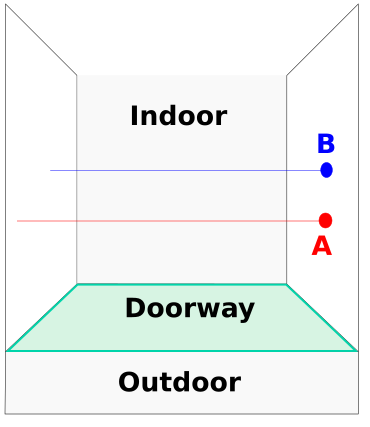
\includegraphics[width=0.3\textwidth]{twoultrasonic.png}
\end{figure}

  Suppose a sensor A, is placed at the front and another sensor B is
  placed at the rear of the doorway so that when a person enters the
  room, sensor A gets triggered first and only then sensor B gets
  triggered.  As a result, the time at which the transmitted signal
  reflects back will be less for sensor A and it implies that a person
  just entered the room. Conversely, when a person leaves the room,
  sensor B gets triggered first, and sensor A gets triggered second
  which implies that a person just left the room.

  One major flaw of this system is that even if more than one people
  enter a room simultaneously the sensors are only able to interpret
  them as a single person. So in order to overcome this limitation, we
  use four ultrasonic sensors in sets of 2 instead of just 2 sensors.

  This four sensor arrangement will also have contribution in
  improving the accuracy of the system. Since width of most doorways
  are not that large, sensors from either set may get triggered at the
  exact same time. In such cases, having an extra sensor will help to
  reduce or completely eliminate errors in counting.

  Here is a schematic representation of arrangement with four sensors:

  \begin{figure}[H]
    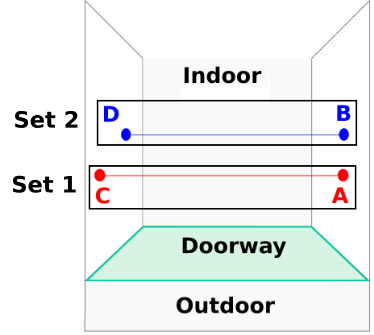
\includegraphics[width=0.4\textwidth,inner]{fourultrasonic.png}
  \end{figure}

  As illustrated earlier, set 1 will be placed at front of the doorway
  and set 2 will be placed at the rear end of the doorway to determine
  whether a person is exiting or entering.

  The logic behind using 4 sensors for estimating the number of people
  walking past the doorway is fairly simple. First we calculate an
  approximate width of the obstacle in the doorway as follows:

\begin{figure}[H]
  \centering
  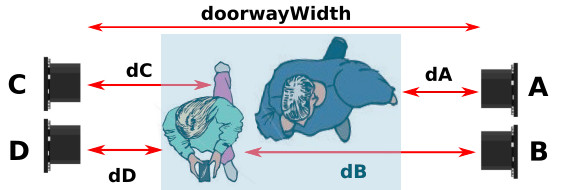
\includegraphics[width=0.5\textwidth]{people-walking-simultaenously.jpeg}
\end{figure}

\verb|obstacleWidth = doorwayWidth -|\newline
\verb|         (min(dA,dC) + min(dB,dD));|

  This ``obstacleWidth'' can be then compared with a standard value to
  predict the possible number of people walking past the doorway.

  \end{multicols}

\subsubsection{Algorithm}

\textbf{Step 1:} Collect data from the sensor

\begin{itemize}

  \item Time values tA, tC, tB and tD are the time-stamps at which the
    respective sensors detects the transmitted sound wave after it
    reflects back.

  \item Distance dA, dC, dB, dD are more or less the length of the
    pulse transmitted from the respective sensors and are proportional
    to tA, tC, tB and tD respectively.

\end{itemize}

\textbf{Step 2:} Count the number of visitors inside the room based on
data obtained from the sensors

\begin{verbatim}
    obstacleWidth = doorwayWidth - (min(dA,dC) + min(dB,dD));

    if (tA < tB || tA < tD || tC < tB || tC < tD)

        if (obstacleWidth > certainStandardValue)
            visitorCount = visitorCount + estimatedPeopleEntering;
          else
            visitorCount++; // at least one person entered

    else if (tB < tA || tB < tC || tD < tA || tD < tC)

        if (obstacleWidth > certainStandardValue)
            visitorCount = visitorCount - estimatedPeopleExiting;
          else
            visitorCount--;
\end{verbatim}

\textbf{Step 3:} Turn the lights off if there is no one inside the
room.
\begin{verbatim}
        if visitorCount == 0 && lightON {
            delay();
            turnOffLights();
          }
\end{verbatim}
\vfill \newpage

\subsection{Home Security System}

Under home security system, our primary goal is to notify the home
about possible leakage of flammable LPG gas via. mobile networking.
This security system serves the sole purpose of notifying the user
about possible fire accidents so that the owner can take necessary
actions to prevent them. In a way, this makes our home just a bit more
secure.

For the sake of this, first we need to determine whether there is a
gas leakage. A gas sensor is a device which detects the presence or
concentration of gases in the atmosphere. Based on the concentration
of the gas, the sensor produces a corresponding potential difference
by changing the resistance of the material inside the sensor, which
can be measured as the output voltage.

Basically, the sensor is designed in such a fashion that whenever it
detects presence of flammable gas in the air, it gets triggered. The
concentration of LPG gas detected won't matter as much because in
normal air its concentration is usually 0. Once the sensor has been
triggered, it sends a signal to the microcontroller unit.

The second part of this design, is notifying the user about the
leakage that has just been detected. This is done via. mobile
networking. A GSM module is interfaced with the microcontroller such
that it broadcasts a predefined message to user in the form of an SMS
as an alert signal about the leakage on his/her cell phone.

\subsubsection{Algorithm}

\textbf{Step 1:} Acquire a signal form the sensor.

\textbf{Step 2:} If the leakage is detected notify the user via SMS.

\begin{verbatim}
    if (leakageSensorSignalHigh)
        broadcastSMS();
    else
        noop; // no operation
\end{verbatim}

\vfill \newpage
\subsection{Touchless Automatic Trash Can}

The concept of a touchless automatic trash can is also pretty much
straightforward. The first thing that we require is a trash can with a
LID whose lid opens when a foot is placed at the bottom of the trash
can. Now, a PIR sensor is placed at face of this trash can to detect
movement. A servo-motor is placed at the bottom of the trash can just
beside the part where placing a foot would open the trash can.

The PIR sensor detects motion by evaluating fluctuations in the amount
of infrared radiation within a certain range of its proximity. The
infrared radiation impinging upon the PIR sensor varies with respect
to temperature and surface characteristics of the objects right in
front of it.

Living creatures emit certain heat energy in the form of infrared
radiation when they move. Therefore, when someone appears in front of
the sensing element or when ever someone comes within the sensor's
range, the sensor will detect a motion by sensing fluctuations in
temperature or the amount of IR radiation in that region. The sensor
converts the resulting change in infrared radiation into a change in
the output voltage, and transmits it to the controlling unit. When the
microcontroller receives such signal from the PIR sensor, it will
deploy a output signal of certain magnitude, which sets the servo
motor interfaced with in into motion, allowing the trash can's lid to
open automatically.

Finally, if the person in front of the sensor moves away, the
parameters around the environment will get restored and the sensor
will stop transmitting a signal to the controller.

\subsubsection{Algorithm}

\textbf{Step 1:} Acquire a signal form the sensor.

\textbf{Step 2:} Send a pulse to the external circuit to turn the
server motor if the signal from the sensor is high.

\begin{verbatim}
    if (motionSensorSignalHigh)
        transmitSignalToPowerMotor();
\end{verbatim}
\textbf{Step 3:} The trash can has an auto closing mechanism so there
is no need to perform anything to close the lid. If the sensor signal
is low simply halt the signal from the controller so that the servo
motor turns off.

\begin{verbatim}
    if (motionSensorSignalLow)
        stopSignalPoweringMotor();
\end{verbatim}

\newpage
\section{Block-diagram and Overall Circuitry}

Block-diagram of the proposed system:

\begin{figure}[H]
  \centering
  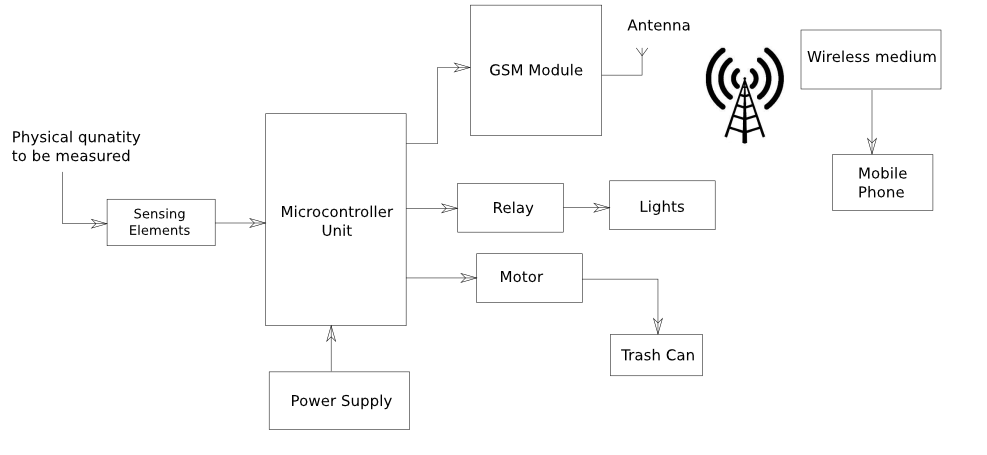
\includegraphics[width=\textwidth]{block-diagram}
\end{figure}

As seen in the block diagram the micro-controller will be the heart of the system.

A schematic circuit representation of the system is as follows:

\begin{figure}[H]
  \centering
  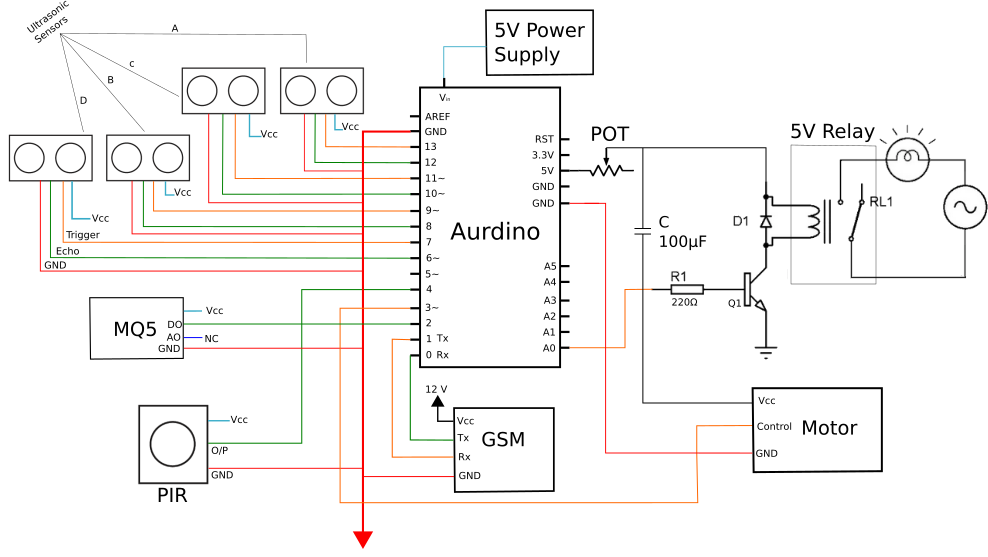
\includegraphics[width=\textwidth]{schematic-ckt}
\end{figure}
\newpage

